%% abtex2-modelo-trabalho-academico.tex, v-1.8 laurocesar
%% Copyright 2012-2013 by abnTeX2 group at http://abntex2.googlecode.com/ 
%%
%% This work may be distributed and/or modified under the
%% conditions of the LaTeX Project Public License, either version 1.3
%% of this license or (at your option) any later version.
%% The latest version of this license is in
%%   http://www.latex-project.org/lppl.txt
%% and version 1.3 or later is part of all distributions of LaTeX
%% version 2005/12/01 or later.
%%
%% This work has the LPPL maintenance status `maintained'.
%% 
%% The Current Maintainer of this work is the abnTeX2 team, led
%% by Lauro César Araujo. Further information are available on 
%% http://abntex2.googlecode.com/
%%
%% This work consists of the files abntex2-modelo-trabalho-academico.tex,
%% abntex2-modelo-include-comandos and abntex2-modelo-references.bib
%%

% ------------------------------------------------------------------------
% ------------------------------------------------------------------------
% abnTeX2: Modelo de Trabalho Academico (tese de doutorado, dissertacao de
% mestrado e trabalhos monograficos em geral) em conformidade com 
% ABNT NBR 14724:2011: Informacao e documentacao - Trabalhos academicos -
% Apresentacao
% ------------------------------------------------------------------------
% ------------------------------------------------------------------------

\documentclass[
	% -- opções da classe memoir --
	11pt,				% tamanho da fonte
	openright,			% capítulos começam em pág ímpar (insere página vazia caso preciso)
	oneside,			% twoside para impressão em verso e anverso. Oposto a oneside
	a4paper,			% tamanho do papel. 
	% -- opções da classe abntex2 --
	%chapter=TITLE,		% títulos de capítulos convertidos em letras maiúsculas
	%section=TITLE,		% títulos de seções convertidos em letras maiúsculas
	%subsection=TITLE,	% títulos de subseções convertidos em letras maiúsculas
	%subsubsection=TITLE,% títulos de subsubseções convertidos em letras maiúsculas
	% -- opções do pacote babel --
	english,			% idioma adicional para hifenização
	french,				% idioma adicional para hifenização
	spanish,			% idioma adicional para hifenização
	brazil,				% o último idioma é o principal do documento
	]{abntex2}

\usepackage{Pacotes/abntex2-cefetmg-timoteo}

% ---
% PACOTES
% ---

% ---
% Pacotes fundamentais 
% ---
\usepackage{cmap}				% Mapear caracteres especiais no PDF
\usepackage{lmodern}			% Usa a fonte Latin Modern			
\usepackage[T1]{fontenc}		% Selecao de codigos de fonte.
\usepackage[utf8]{inputenc}		% Codificacao do documento (conversão automática dos acentos)
\usepackage{lastpage}			% Usado pela Ficha catalográfica
\usepackage{indentfirst}		% Indenta o primeiro parágrafo de cada seção.
\usepackage{color}				% Controle das cores
\usepackage{graphicx}			% Inclusão de gráficos
\PassOptionsToPackage{normalem}{ulem} % Para não usar sublinhado em referências bibliográficas
\usepackage{ulem}
\usepackage{multicol}
% ---

%Trocar fonte para Arial ou Helvetica
%\usepackage{uarial}
\usepackage{helvet}
\renewcommand{\familydefault}{\sfdefault}

		
% ---
% Pacotes adicionais, usados apenas no âmbito do Modelo Canônico do abnteX2
% ---
%\usepackage{lipsum}				% para geração de dummy text
% ---

% ---
% Pacotes de citações
% ---
\usepackage[brazilian,hyperpageref]{backref}	 % Paginas com as citações na bibl
\usepackage[alf,abnt-thesis-year=both,]{abntex2cite}	% Citações padrão ABNT


%Outros pacotes

\usepackage{longtable}


%\setlrmarginsandblock{3cm}{2cm}{*}
%\setulmarginsandblock{3cm}{2cm}{*}
%\checkandfixthelayout


% --- 
% CONFIGURAÇÕES DE PACOTES
% --- 

% ---
% Configurações do pacote backref
% Usado sem a opção hyperpageref de backref
\renewcommand{\backrefpagesname}{Citado na(s) página(s):~}
% Texto padrão antes do número das páginas
\renewcommand{\backref}{}
% Define os textos da citação
\renewcommand*{\backrefalt}[4]{
	\ifcase #1 %
		Nenhuma citação no texto.%
	\or
		Citado na página #2.%
	\else
		%Citado #1 vezes nas páginas #2.%
		Citado nas páginas #2.%
	\fi}%
% ---


% ---
% Informações de dados para CAPA e FOLHA DE ROSTO
% ---
\titulo{Comparação entre modelos de tradução neurais de código aberto}
\autor{Marcos Vinícius de Oliveira Silva}
\local{Timóteo}
\data{2026}
\orientador{Douglas Nunes de Oliveira}
\coorientador{}
\instituicao{%
  Centro Federal de Educação Tecnológica de Minas Gerais
  \par
  Campus Timóteo
  \par
  Graduação em Engenharia de Computação
}
\tipotrabalho{Trabalho de conclusão de curso (Graduação)}
% O preambulo deve conter o tipo do trabalho, o objetivo, 
% o nome da instituição e a área de concentração 

%\preambulo{Proposta de pesquisa apresentada à Coordenação de Engenharia de Computação do Campus Timóteo do Centro Federal de Educação Tecnológica de Minas Gerais para obtenção do grau de Bacharel em Engenharia de Computação.}

\preambulo{Monografia apresentada à Coordenação de Engenharia de Computação do Campus Timóteo do Centro Federal de Educação Tecnológica de Minas Gerais para obtenção do grau de Bacharel em Engenharia de Computação.}

% ---

% ---
% Configurações de aparência do PDF final

% informações do PDF
\makeatletter
\hypersetup{
     	%pagebackref=true,
		pdftitle={\@title}, 
		pdfauthor={\@author},
    	pdfsubject={\imprimirpreambulo},
	    pdfcreator={LaTeX with abnTeX2},
		pdfkeywords={abnt}{latex}{abntex}{abntex2}{trabalho acadêmico}, 
		colorlinks=true,       		% false: boxed links; true: colored links
    	linkcolor=black,          	% color of internal links
    	citecolor=black,        		% color of links to bibliography
    	filecolor=black,      		% color of file links
		urlcolor=black,
		bookmarksdepth=4
}
\makeatother
% --- 

% --- 
% Espaçamentos entre linhas e parágrafos 
% --- 

% O tamanho do parágrafo é dado por:
\setlength{\parindent}{1.3cm}

% Controle do espaçamento entre um parágrafo e outro:
\setlength{\parskip}{0.2cm}  % tente também \onelineskip

% ---
% compila o indice
% ---
\makeindex
% ---

% ----
% Início do documento
% ----
\begin{document}

% Retira espaço extra obsoleto entre as frases.
\frenchspacing 

% ----------------------------------------------------------
% ELEMENTOS PRÉ-TEXTUAIS
% ----------------------------------------------------------
 \pretextual

% ---
% Capa
% ---
\imprimircapa
% ---

% ---
% Folha de rosto
% (o * indica que haverá a ficha bibliográfica)
% ---
\imprimirfolhaderosto*
% ---

% ---
% Inserir a ficha bibliografica
% ---

% Isto é um exemplo de Ficha Catalográfica, ou ``Dados internacionais de
% catalogação-na-publicação''. Você pode utilizar este modelo como referência. 
% Porém, provavelmente a biblioteca da sua universidade lhe fornecerá um PDF
% com a ficha catalográfica definitiva após a defesa do trabalho. Quando estiver
% com o documento, salve-o como PDF no diretório do seu projeto e substitua todo
% o conteúdo de implementação deste arquivo pelo comando abaixo:
%
% \begin{fichacatalografica}
%		\includegraphics{inclusao-fichaCatalografica.pdf}
% \end{fichacatalografica}
%\begin{fichacatalografica}
%	\vspace*{\fill}					% Posição vertical
%	\hrule							% Linha horizontal
%	\begin{center}					% Minipage Centralizado
%	\begin{minipage}[c]{12.5cm}		% Largura
%	
%	\imprimirautor
%	
%	\hspace{0.5cm} \imprimirtitulo  / \imprimirautor. --
%	\imprimirlocal, \imprimirdata-
%	
%	\hspace{0.5cm} \pageref{LastPage} p. : il. (algumas color.) ; 30 cm.\\
%	
%	\hspace{0.5cm} \imprimirorientadorRotulo~\imprimirorientador\\
%	
%	\hspace{0.5cm}
%	\parbox[t]{\textwidth}{\imprimirtipotrabalho~--~\imprimirinstituicao,
%	\imprimirdata.}\\
%	
%	\hspace{0.5cm}
%		1. Palavra-chave1.
%		2. Palavra-chave2.
%		I. Orientador.
%		II. Universidade xxx.
%		III. Faculdade de xxx.
%		IV. Título\\ 			
%	
%	\hspace{8.75cm} CDU 02:141:005.7\\
%	
%	\end{minipage}
%	\end{center}
%	\hrule
%\end{fichacatalografica}
% ---

% ---
% Inserir errata
% ---
\input{1-Pre-Textual/Errata.tex}
% ---


% ---
% Inserir folha de aprovação
% ---
%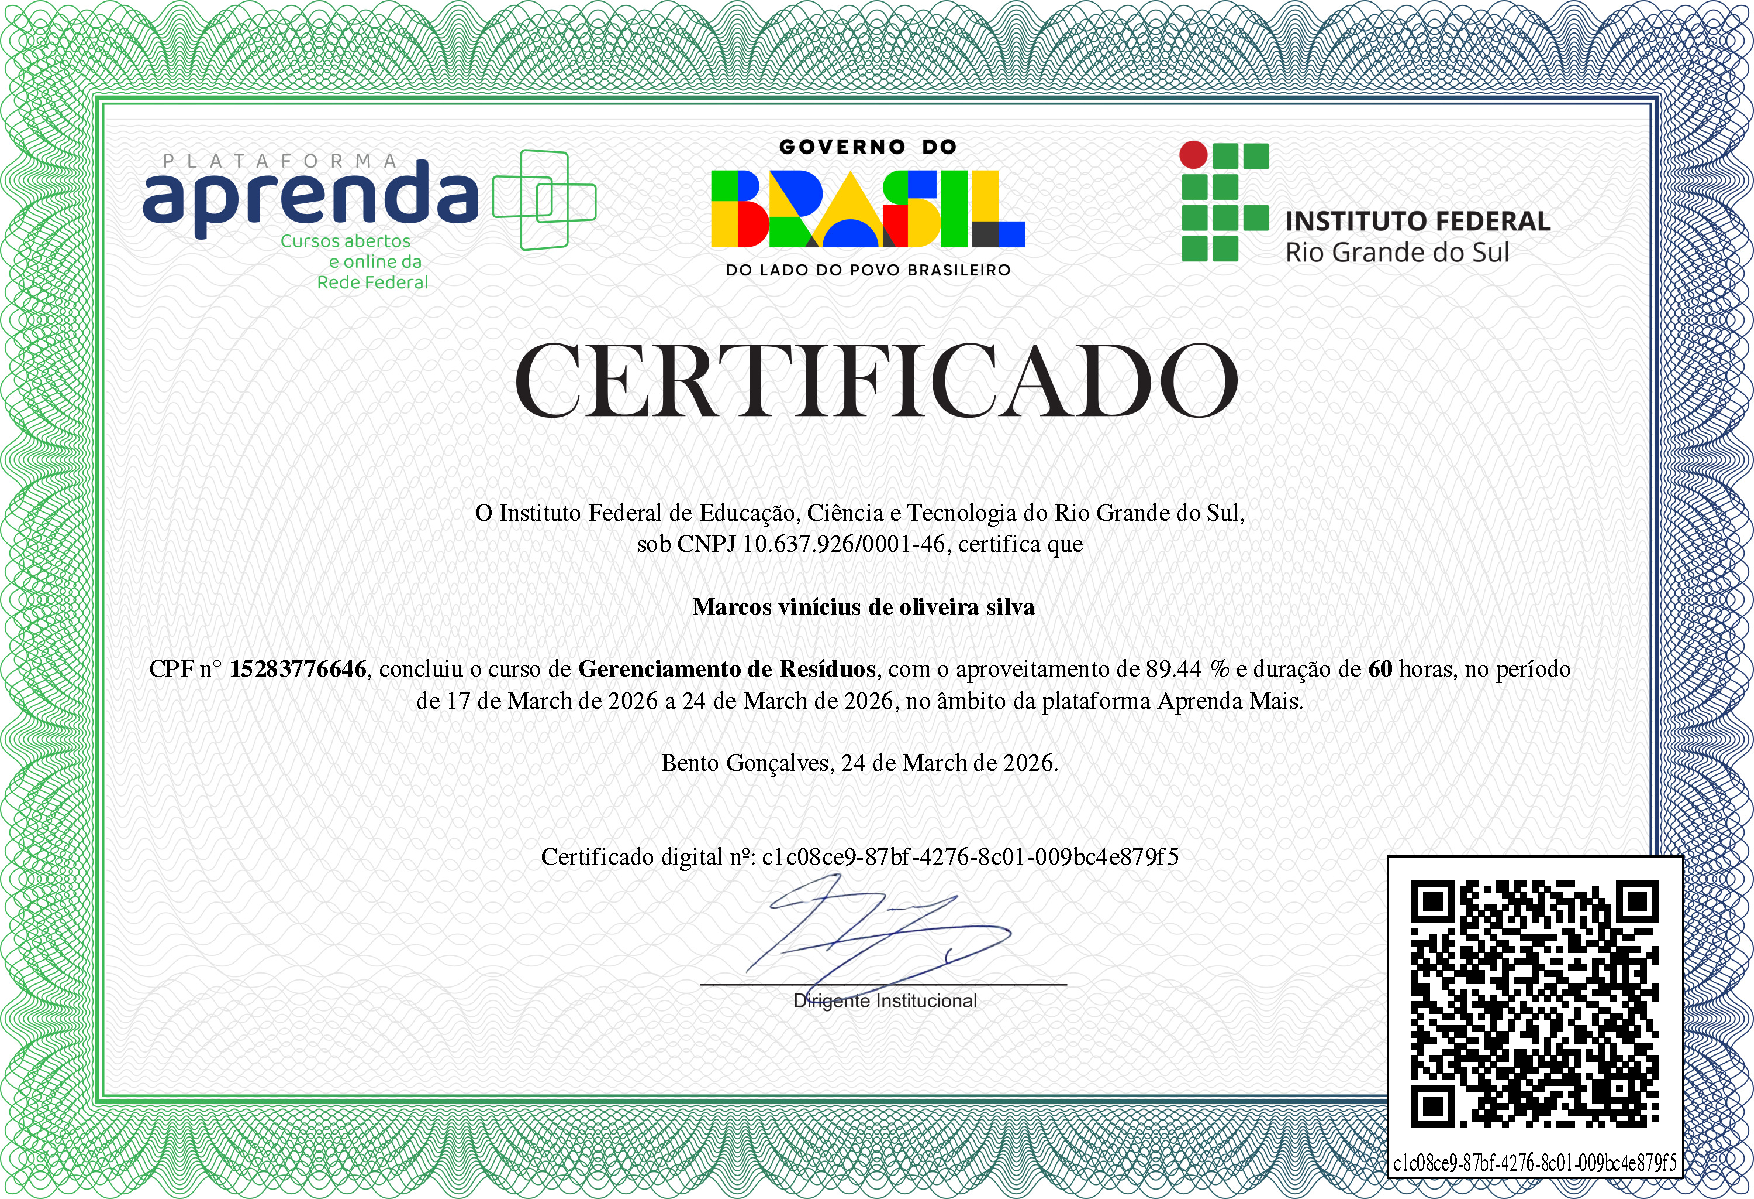
\includegraphics[width=1\textwidth]{Imagens/Gerenciamento_de_Residuos-Certificado_digital_3881527.pdf}
%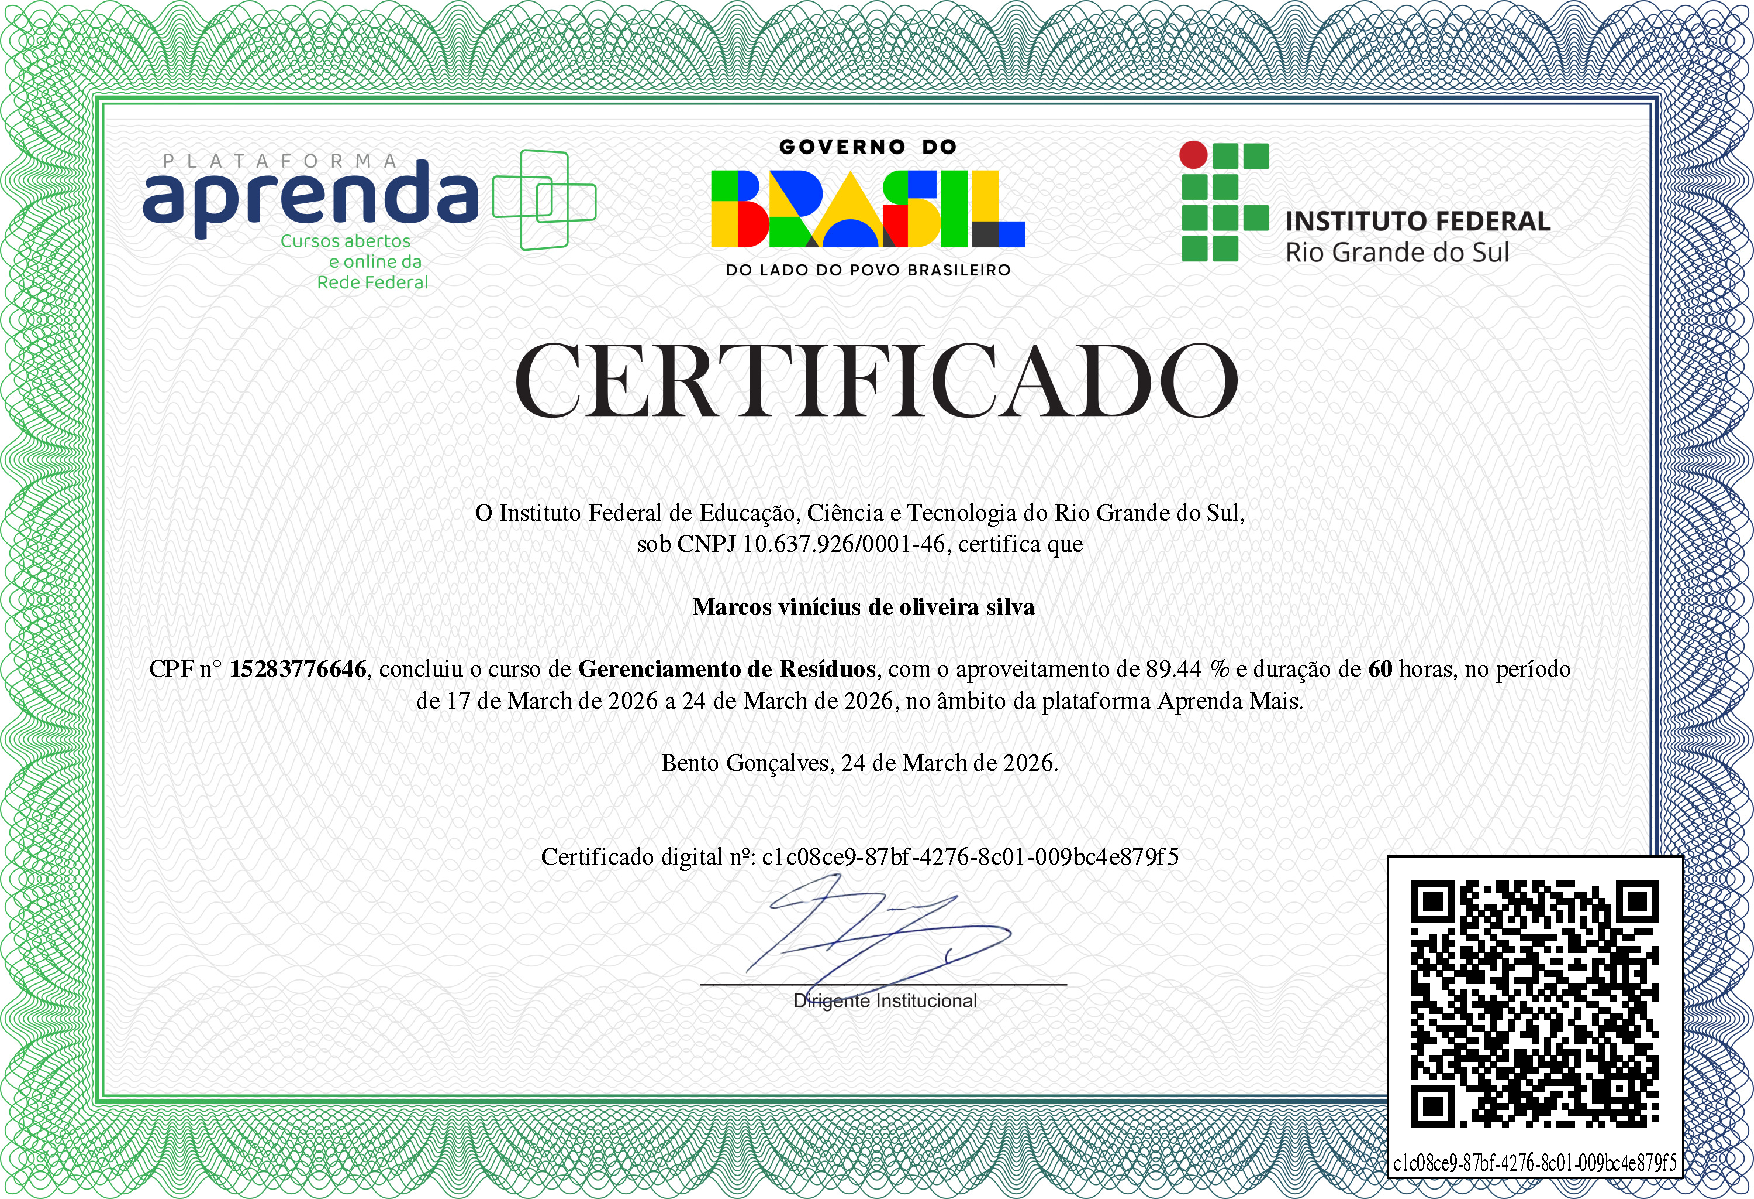
\includegraphics[width=1\textwidth]{Imagens/Gerenciamento_de_Residuos-Certificado_digital_3881527.pdf}
% ---


% ---
\newpage
% ---
% Dedicatória
% ---
\begin{dedicatoria}
    \vspace*{\fill}
	\begin{flushright}
		À, Jonas Garcia de Oliveira, colega, amigo e avô
	\end{flushright}
\end{dedicatoria}
% ---


% ---
% Agradecimentos
% ---
\begin{agradecimentos}

Agradeço aos pais no primeiro parágrafo?

E à namorada ou ao namorado no segundo?

Orientador no terceiro?

Esta página de agradecimentos vive dando problemas.

\end{agradecimentos}
% ---


% ---
% Epígrafe
% ---
\begin{epigrafe}
    \vspace*{\fill}
	\begin{flushright}
		\textit{``Por pior que a vida pareça, sempre existe algo que você possa fazer e ser bem-sucedido''.\\
		Stephen Hawking}
	\end{flushright}
\end{epigrafe}
% ---

% ---
% RESUMO EM PORTUGUÊS
% ---
\setlength{\absparsep}{18pt}
Um único parágrafo que sintetize todo o meu trabalho. Organização de informação usando classificação facetada é útil para melhorar a indexação de documentos e a construção de sistemas de recuperação de informação corporativa. Essa hipótese baseia-se na evidência de facetas comuns a documentos de diferentes empresas e na flexibilidade da organização facetada. Entretanto, a classificação e indexação automáticas de um grande volume de documentos representam importantes obstáculos e nossa principal motivação. A pesquisa é descritiva, aplicada e experimental e tenta responder sobre a existência de características comuns a documentos do domínio corporativo e a possibilidade de indexação facetada automática. Duas coleções são usadas para avaliação, uma pública e outra particular. Os termos usados por autores de documentos foram obtidos através de documentos e expressões de busca. Foi empreendida uma análise preliminar do domínio corporativo, pela qual foram descobertas 12 categorias comuns e facetas úteis para o contexto de cada coleção de avaliação. A distribuição de assuntos em categorias apresentou alta correlação positiva usando o coeficiente de correlação de Spearman. Dez expressões de busca de usuários foram avaliadas no contexto da coleção particular e validaram as 12 categorias comuns. A avaliação empírica da trilha \textit{Enterprise} da \textit{Text Retrieval Conference} foi executada e os métodos de indexação, classificação e recuperação automáticos de informação facetada melhoraram a eficiência da recuperação sem fazer uso de serviços externos, como Wikipedia e metabuscadores, e sem fazer uso de estruturas hipertextuais presentes nos documentos da amostra. A avaliação empírica utilizou-se principalmente das características espaciais, temporais, de documento e de pessoal. A técnica de análise facetada mostrou-se promissora para os métodos de análise e comparação de coleções corporativas sem que dados puros sejam expostos a terceiros. A tese aponta direções de pesquisa para o uso dos métodos em outras coleções, para aperfeiçoamentos da organização da informação facetada, e para novas aplicações dos métodos também em outros domínios.
% ---

% ---
% RESUMO EM INGLÊS
% ---
We hypothesise that information organisation based on faceted classification is useful to improve enterprise information retrieval systems. The existence of similar facets in documents from different companies and the known adaptability of facet organisation strengthen this hypothesis. We refer this work to the automated classification and indexing on large amounts of text files. This work is descriptive, applied, and experimental. It aimed to expose the main characteristics of the enterprise information, proposing a tentative generalisation to the enterprise domain and presenting some facets we can use to organise it and to support better information retrieval. It applied facet analysis to two enterprise collections and evaluated the resulting faceted classification. Terms were selected from documents and queries. We found twelve common categories and the distribution of document subjects across the categories presents strong positive correlation by the Spearman’s rank correlation. Then, we obtained ten user queries and we adopted them to validate the found categories. We also used the Enterprise track of Text Retrieval Conference and its previous results as a Cranfield-like evaluation. The automated prototype used spatial, temporal, document and social characteristics. Thus, our empirical evaluation improved the information retrieval with no external dependency like Wikipedia or metasearch engines. The facet analysis was useful for comparing the companies with no desire to expose their information. The method can guide and stimulate future work and other companies can become more willing to take part in a research study.
% ---


% ---
% inserir lista de ilustrações
% ---

%%% no extra space before the entry, or in the LoF/LoT
% \setlength{\cftbeforechapterskip}{0pt plus 0pt} %afeta sumário, o que não desejo!
 \renewcommand*{\insertchapterspace}{} %afeta apenas lista de figuras e lista de tabelas, precisamente o que desejo!

\pdfbookmark[0]{\listfigurename}{lof}
\listoffigures*
\cleardoublepage
% ---

% ---
% inserir lista de tabelas
% ---
\pdfbookmark[0]{\listtablename}{lot}
\listoftables*
\cleardoublepage
% ---


% ---
% inserir lista de símbolos
% ---
\input{1-Pre-Textual/Simbolos.tex}
% ---


% ---
% inserir lista de abreviaturas e siglas
% ---
\chapter*{Lista de Abreviaturas e Siglas}
\begin{acronym}[xxxxxxxxx]
    \acro{API}{Interface de Programação de Aplicativos, do inglês \textit{Application Programming Interface}}
    \acro{CPU}{Unidade Central de Processamento, do inglês \textit{Central Processing Unit}}
    \acro{DAG}{Grafos Acíclicos Dirigidos, do inglês \textit{Directed Acyclic Graph}}
    \acro{GC}{Coletor de Lixo, do inglês \textit{Garbage Collector}}
    \acro{VM}{Maquina Virtual, do inglês \textit{Virtual Machine}}
\end{acronym}
% ---

% ---
% inserir o sumario
% ---
\pdfbookmark[0]{\contentsname}{toc}
\tableofcontents*
\cleardoublepage
% ---



% ----------------------------------------------------------
% ELEMENTOS TEXTUAIS
% ----------------------------------------------------------
\textual

% ----------------------------------------------------------
% Introdução
% ----------------------------------------------------------
\chapter[Introdução]{Introdução}

%\chapter{Introdução}

%\textbf{Organização de informação não se dá da mesma forma em qualquer domínio.}
O mundo passou e vem passando por grandes mudanças tecnologicas nos ultimos anos, o que possibitou a presença da tecnologia em diversos setores econômicos \cite{del2009avancco}. Juntamente com a presença tecnologica as pessoas puderam se tornar mais ativos virtualmente, uma vez que a tecnologia faz parte do dia a das pessoas e em conjunto com essa presença digital se tornou notável o consumo de conteúdos de outros páises




\section{Justificativa} %Inseri para organizar o texto

Hoje em dia existem diversos modelos neurais de tradução de código aberto, porém cada modelo possui dados de trinamento diferentes, e por mais que todos os modelos presentados neste trabalho sejam baseados na arquietura transformer, cada modelo terá caracteristicas arquiteturais que irão diferenciar um modelo do oytro, impactando o resultado final da tarefa de tradução.Este trabalho visa comaparara cada modelo a fim de mostrar onde e porque cada modelo se sobressaí em relação ao outro quando se trata de uma tarefa de tradução. 

\section{Problema}

A seguinte questão constitue o problema desta pesquisa: 
Qual é o desempenho de diferentes modelos de tradução entre línguas e automática, baseados na arquitetura Transformer para a tarefa de tradução do inglês para o português, considerando métricas como consumo de memória, uso de CPU, pontuação BLEU, BERTScore e chrF, em diferentes cenários de teste?


\section{Objetivos}

%\textbf{Objetivo geral.}
Para responder ao problema proposto, o objetivo geral deste trabalho é investigar e comparar o desempenho de modelos de tradução entre línguas e automática baseados na arquitetura Transformer na tarefa de tradução do inglês para o português, considerando métricas de qualidade (BLEU, BERTScore e chrF) e eficiência computacional (uso de memória e CPU) em diferentes cenários experimentais.

Também, objetivam-se mais especificamente:

\begin{enumerate}
	\item Revisão bibliográfica sobre o funcionamento de modelos de tradução automática neural baseados na arquitetura Transformer;

	\item Selecionar e configurar os modelos de tradução automática neural de código aberto;

	\item Selecionar base de dados pública para comparação entre os modelos de tradução automática neural;
	
    \item Avaliar qualidade de tradução utilizando metricas como BLEU, BERTScore e chrF;
    
    \item Medir eficiência de recursos computacionais quando se utiliza modelos de tradução;
    
    \item Avaliar os modelos de tradução diferentes cenários de teste;
    
    \item Analisar correlação entre métricas de qualidade de tradução.

\end{enumerate}






% ----------------------------------------------------------
% Estado da arte/história
% ----------------------------------------------------------
\chapter{Evolução modelos de tradução}
A área de tradução automática tem passado por transformações significativas ao longo dos anos, seja pela evolução de modelos específicos por meio de técnicas de otimização, seja pela proposição de novas arquiteturas que estabeleceram novos estados da arte. Este capítulo tem como objetivo apresentar um panorama da evolução das técnicas e modelos de tradução automática, desde as abordagens iniciais até os métodos mais recentes, discutindo suas principais características, vantagens e limitações.

\section{Tradução Automática Baseada em Regras}
A tradução automática baseada em regras, do inglês Rule-Based Machine Translation (RBMT), consiste em sistemas que operam com base em um conjunto de regras linguísticas previamente definidas para a língua de destino. Esses sistemas utilizam regras gramaticais para realizar a tradução entre línguas, exigindo um esforço humano significativo na elaboração de todos os componentes necessários para a tradução de uma língua de origem para uma língua de destino.

Entre esses componentes, destacam-se analisadores morfológicos, etiquetadores de classes gramaticais, analisadores sintáticos, dicionários bilíngues, regras de transferência, geradores morfológicos e regras de reordenação, entre outros \cite{DBLP:journals/corr/abs-1708-04559}.

A Figura \ref{fig:rbmt-processo} ilustra o processo de tradução baseado em regras. Nela, uma frase em inglês é fornecida para o sistema, e baseado nas regras pre-definidas da língua portuguesa como língua de destino a tradução é gerada.

\begin{figure}[H]
	\caption{\label{fig:rbmt-processo}Tradução Automática Baseada em Regras}

	\centering
		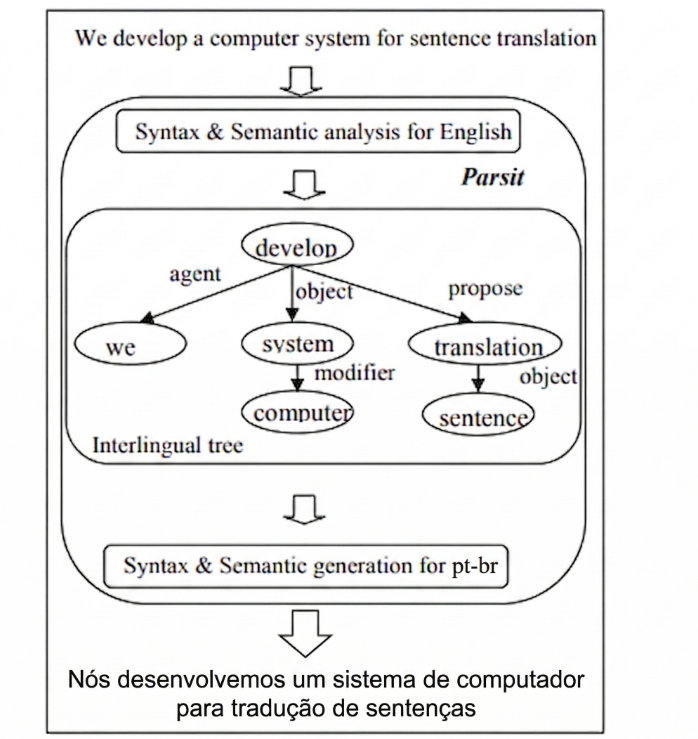
\includegraphics[width=.80\textwidth]{Imagens/RBMT-estado-da-arte.png}

	\legend{Fonte: \cite{charoenpornsawat2002improving} adaptada para português}
\end{figure}

A tradução automática baseada em regras teve início na década de 1970, sendo considerada um marco na área de tradução automática e uma abordagem inicialmente promissora \cite{wiki:Rule-based_machine_translation}. No entanto, algumas características limitaram sua adoção em larga escala \cite{okpor2014machine}:

\begin{itemize}
    \item Escassez de dicionários bilíngues de alta qualidade, sendo sua construção uma tarefa custosa;
    \item Necessidade de configuração manual de diversas informações linguísticas;
    \item Dificuldade em lidar com ambiguidade linguística e expressões idiomáticas, especialmente em sistemas de grande escala.
\end{itemize}

Devido a essas limitações, tornou-se necessária a criação de novas abordagens capazes de lidar melhor com ambiguidade, dependências contextuais entre palavras e reduzir a necessidade de intervenção humana na construção das traduções. Nesse contexto, surgiu a tradução automática baseada em Estatística (Statistical Machine Translation – SMT), que será abordada na na próxima seção.


\section{Tradução Automática Estatística}
A abordagem estatística de tradução baseia-se em modelos probabilísticos extraídos de bases textuais bilíngues alinhadas, nos quais cada palavra ou frase da língua de destino é associada a elementos da língua de origem segundo uma determinada probabilidade. Dessa forma, as palavras ou expressões com maior probabilidade, dentre as opções geradas pelo modelo, tendem a corresponder à tradução mais adequada \cite{DBLP:journals/corr/abs-1708-04559}.

Em termos práticos, um modelo de tradução estatística é treinado com grandes volumes de textos paralelos, contendo a língua de origem e sua tradução correspondente na língua de destino. A partir desses dados, o modelo aprende padrões de correspondência entre palavras e frases, sendo capaz de estimar a tradução mais provável com base nas ocorrências observadas durante o treinamento \cite{lokalise_smt_2025}.

O processo de tradução estatística envolve dois módulos principais: o modelo de tradução e o modelo de linguagem \cite{wang2017neural}.

O modelo de tradução tem como objetivo mapear como palavras ou frases em uma língua geralmente se correspondem em outra, realizando essa análise no nível de frases, e não apenas de palavras isoladas. Esse cuidado evita traduções que não respeitem o contexto, já que uma mesma palavra na língua de origem pode ter múltiplas traduções possíveis na língua de destino.

O modelo de linguagem, por sua vez, recebe os possíveis mapeamentos gerados pelo modelo de tradução e seleciona a frase que apresenta a maior probabilidade de ocorrência na língua de destino, considerando padrões aprendidos a partir dos textos da base de observação. Esse módulo é essencial para produzir traduções mais naturais, que se aproximem do resultado esperado de uma tradução humana.

A imagem abaixo exemplifica este processo de tradução baseado no modelo estatístico. 

\begin{figure}[H]
	\caption{\label{fig:smt-processo}Tradução Automática Baseada em estatística}

	\centering
		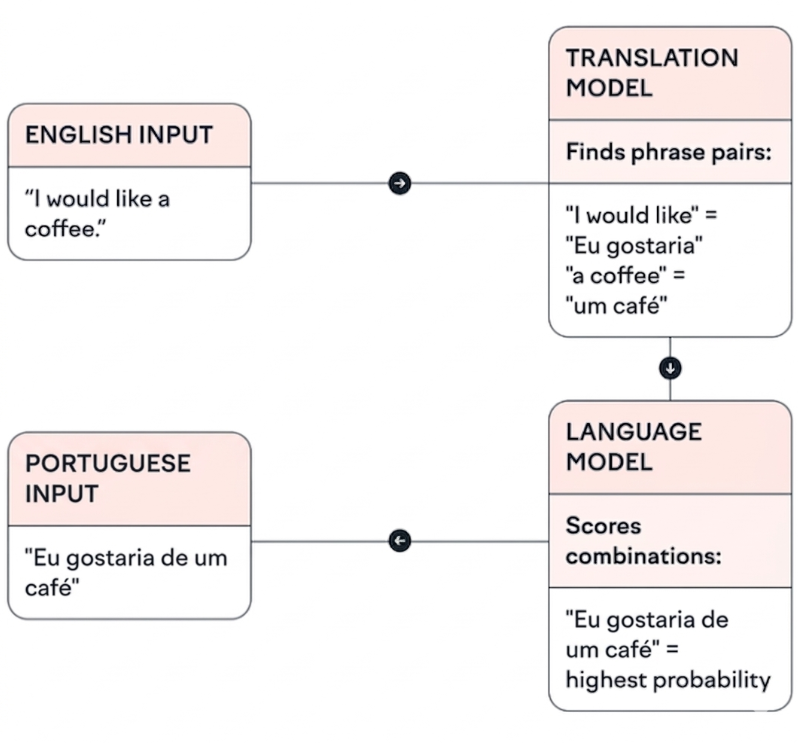
\includegraphics[width=.80\textwidth]{Imagens/estatistica-estado-arte.png}

	\legend{Fonte: \cite{lokalise_smt_2025} adaptada para português}
\end{figure}

É notável que traduções baseadas em estatística superaram traduções baseadas em regras, em qualidade e contexto, porém, os seguintes pontos podem ser destacados sobre traduções estatísticas \cite{wang2017neural}:

\begin{itemize}
    \item Criação de base de dados complexa;
    \item Resultados inesperados. Fluência superficial pode ser enganosa;
    \item Tradução baseada em estatística não funciona bem entre línguas que possuem ordem de palavras diferentes;
    \item Os resultados obtidos tendem a ser mais favoráveis para línguas europeias.
    \item Dificuldade em lidar com dependências de longa distância em frases.
\end{itemize}

Para contornar os problemas listados acima, um novo modelo foi proposto, o qual foi a base para construção de modelos utilizados atualmente, conhecido como aprendizado profundo, em inglês, deep learning, que será abordado no próximo capítulo.

\section{Tradução automática neural}

A tradução automática neural, em sua essência, utiliza redes neurais artificiais (Artificial Neural Networks - ANN), cujo objetivo é simular, de forma simplificada, o funcionamento do cérebro humano. Em termos gerais, o sistema recebe uma entrada, neste caso, um texto na língua de origem, e por meio de módulos internos da rede neural, realiza a tradução para a língua de destino \cite{laratranslate2025neural}.

O processo de tradução é realizado por meio de dois componentes principais: o codificador (encoder) e o decodificador (decoder) \cite{wang2022progress}.

O componente de codificação tem como objetivo mapear o texto de entrada em um vetor de valores reais de múltiplas dimensões. Esse vetor representa, de forma abstrata, informações relevantes necessárias para a realização da tradução. A partir dessa representação vetorial, o componente de decodificação utiliza essas informações para gerar o texto correspondente na língua de destino.

De forma geral, o processo de tradução automática neural pode ser descrito pelas seguintes etapas \cite{laratranslate2025neural}:

\begin{itemize}
    \item Conversão das palavras em vetores numéricos;
    \item Processamento desses vetores por meio de uma rede neural com múltiplas camadas;
    \item Geração de uma distribuição de probabilidade para possíveis traduções;
    \item Seleção da tradução mais provável.
\end{itemize}

A Figura \ref{fig:nmt-processo} ilustra o processo de tradução utilizando redes neurais artificiais, destacando os componentes de codificação e decodificação.

\begin{figure}[H]
	\caption{\label{fig:nmt-processo}Tradução automática neural}
	\centering
	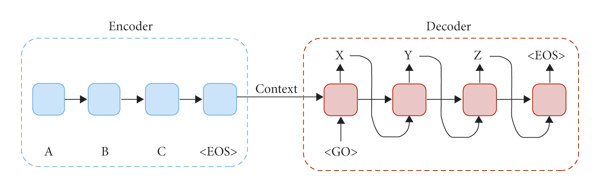
\includegraphics[width=.80\textwidth]{Imagens/encoder-decoder-estado-arte.png}
	\legend{Fonte: \cite{elaffendi2022beyond}}
\end{figure}

O uso da tradução automática neural (Neural Machine Translation – NMT) representou, por muitos anos, uma substituição às técnicas de tradução baseadas em métodos estatísticos. Com a utilização da NMT, tornou-se possível gerar traduções sem a necessidade de intervenção humana direta, baseando-se inteiramente em grandes bases de textos e suas respectivas traduções, abordagem conhecida como aprendizado fim a fim (end-to-end) \cite{laratranslate2025neural}. 

Essa abordagem possibilitou a geração de traduções com maior captura de contexto e maior naturalidade quando comparadas às traduções estatísticas e baseadas em regras, além de melhorar a modelagem das relações entre palavras em uma sentença, um dos principais desafios enfrentados pelas abordagens anteriores \cite{wang2017neural}. 

Um marco importante na adoção da tradução automática neural foi a substituição dos modelos estatísticos pelo uso de NMT no Google Tradutor, realizada pela empresa Google em 2016 \cite{schuster2016zeroshot}, evidenciando uma mudança significativa na forma como sistemas de tradução eram desenvolvidos até então.

Apesar dos avanços proporcionados pela tradução automática neural em relação aos métodos anteriores, ainda existem limitações associadas aos modelos baseados em componentes de codificação e decodificação. Dentre essas limitações, destacam-se \cite{laratranslate2025neural}:

\begin{itemize}
    \item Dificuldade na paralelização do processamento de sequências de entrada;
    \item Limitações no tratamento de dependências de longo alcance entre palavras;
    \item Maior complexidade no processo de treinamento;
    \item Qualidade inferior em determinados cenários de tradução.
\end{itemize}


Com o objetivo de contornar essas limitações, novas abordagens foram propostas, incluindo o uso de mecanismos de atenção, melhorias na paralelização e, posteriormente, o desenvolvimento da arquitetura Transformer.\cite{DBLP:journals/corr/VaswaniSPUJGKP17} 

Dessa forma, o próximo capítulo tem como objetivo apresentar essas abordagens, bem como conceitos relacionados que contribuem para o entendimento da evolução dos modelos de tradução automática neural até os modelos mais recentes, que apresentam elevado desempenho na tarefa de tradução entre línguas.






\chapter{Procedimentos metodológicos}
\input{metodologia.tex}

\chapter{Fundamentos históricos, teóricos e metodológicos}
\input{literatura.tex}

\chapter{Análise de domínio corporativo}
\label{analiseDominio}
\input{analiseDominio.tex}

% ---
% Finaliza a parte no bookmark do PDF, para que se inicie o bookmark na raiz
% ---
\bookmarksetup{startatroot}% 
% ---

% ---
% Conclusão
% ---
\chapter[Conclusão]{Conclusão}
\label{conclusao}
\input{conclusao.tex}


% ----------------------------------------------------------
% ELEMENTOS PÓS-TEXTUAIS
% ----------------------------------------------------------
\postextual


% ----------------------------------------------------------
% Referências bibliográficas
% ----------------------------------------------------------
\bibliography{bibfile}

% ----------------------------------------------------------
% Glossário
% ----------------------------------------------------------
%
% Consulte o manual da classe abntex2 para orientações sobre o glossário.
%
%\glossary

% ----------------------------------------------------------
% Apêndices
% ----------------------------------------------------------

% ---
% Inicia os apêndices
% ---
%\begin{apendicesenv}

% Imprime uma página indicando o início dos apêndices
%\partapendices

% ----------------------------------------------------------
%\chapter{Quisque libero justo}
% ----------------------------------------------------------

%\lipsum[50]

% ----------------------------------------------------------
%\chapter{Nullam elementum urna vel imperdiet sodales elit ipsum pharetra ligula
%ac pretium ante justo a nulla curabitur tristique arcu eu metus}
% ----------------------------------------------------------
%\lipsum[55-57]

%\end{apendicesenv}
% ---


% ----------------------------------------------------------
% Anexos
% ----------------------------------------------------------

% ---
% Inicia os anexos
% ---
%\begin{anexosenv}

% Imprime uma página indicando o início dos anexos
%\partanexos


%\end{anexosenv}

%---------------------------------------------------------------------
% INDICE REMISSIVO
%---------------------------------------------------------------------

%\printindex

\end{document}
